\documentclass[dvipdfmx,a4paper]{jreport} % dvipdfmxオプションを追加
\usepackage{amsmath,amssymb}
\usepackage{graphicx}
\usepackage{url} % ウェブサイトのURLをきれいに表示するため
\usepackage{multicol} % 必要であれば多段組用
\usepackage{caption} % 図表のキャプション設定
\usepackage{subcaption} % subfigure環境用
\usepackage{float} % [H]オプションを使うため

% 日本語設定
\usepackage[utf8]{inputenc}
\usepackage[T1]{fontenc}
\usepackage{otf}
\usepackage[ipaex]{pxchfon} % IPAexフォントを使用 (pxgothicの代わりに推奨)
\usepackage{url}
\usepackage{booktabs}
\usepackage{geometry}
\geometry{a4paper,
    top=30mm,
    bottom=30mm,
    left=25mm,
    right=25mm
}

% タイトルページの作成
\makeatletter
\def\titlepage{%
\thispagestyle{empty}%
\begin{center}%
    \vspace*{\fill}%
    {\huge \bfseries 船舶の抵抗試験に関する実験レポート \\}%
    \vspace{2cm}%
    {\large 実施日時:6月30日\\}%
    \vspace{1cm}%
    {\large 2班\\}%
    \vspace{1cm}%
    {\large 学籍番号:08C23031\\}%
    \vspace{1cm}%
    {\large 氏名:古賀 光一朗 \\}%
    \vspace*{\fill}%
\end{center}%
}
\makeatother

\begin{document}

\titlepage

---

\chapter{目的}
本実験は、ある模型船について抵抗試験を行い、船体周りの流れの状態等を観察するとともに、1+Kを用いた、いわゆる3次元外挿法により想定実船の有効馬力を推定することを目的とする。

---

\chapter{方法}
\section{実験場所および装置}
本実験は、大阪大学工学部地球総合工学科船舶海洋工学科目にある回流水槽にて実施した。主な設備仕様は以下の通りである。

\begin{itemize}
    \item \textbf{回流水槽:} V2-5A SUSという2インペラ方式垂直循環型回流水槽を使用し、約 $1.0~m/s$ の流速を発生することができる。水面加速装置も装備されている。
\end{itemize}

図\ref{fig:recirculating_water_channel}に回流水槽の概略図を示す。

\begin{figure}[H] % floatパッケージのHオプションを使用
    \centering
    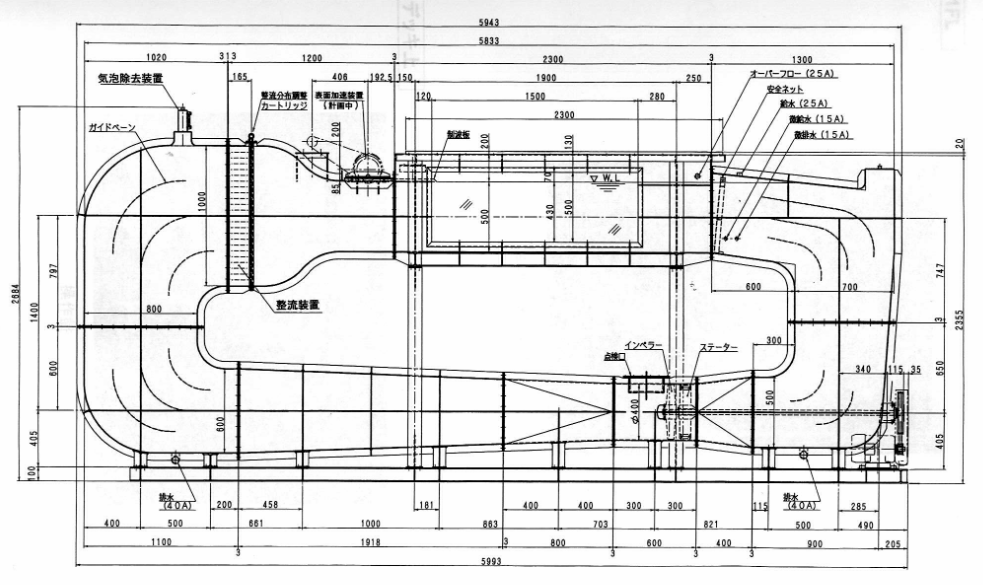
\includegraphics[width=0.8\textwidth]{summer/ship-experiment/circulating-water-channel/recirculating_water_channel.png} 
    \caption{回流水槽概略図}
    \label{fig:recirculating_water_channel}
\end{figure}

計測装置として以下のものを使用した。
\begin{itemize}
    \item \textbf{翼車式流速計:} 模型船の対水速度を計測するための装置である。翼車(プロペラ)の回転数を計測することで、流速を求める。パルスカウンターが付属している。今回使用した流速計はVOT2-100-05Nである。
    \item \textbf{検力計(ロードセル):} 金属棒に力が加わったとき、その金属棒が曲がり、その曲がりを歪みゲージを用いて検出することにより、力を計るものである。歪みゲージの出力をアンプによって増幅し、記録する。
    \item \textbf{サーマルオシロ:} ロードセルからの出力電圧を取り込み、表示・記録を行う。
\end{itemize}

図\ref{fig:load_cell_internal}にロードセルの内部構造を、図\ref{fig:load_cell_setup}に検力計、曳引ロッドと曳航点の位置関係を示す。抵抗試験での曳航点の位置は、プロペラ軸の延長線上とすることが通例であるが、本計測では模型船が小さいため、曳引ロッドを所定の位置に置くことができない。通常と異なる位置に曳航点を設置しているが、これはあくまで便宜的措置である。

\begin{figure}[H]
    \centering
    \begin{subfigure}[b]{0.45\textwidth}
    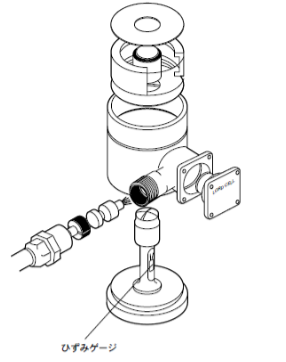
\includegraphics[width=\textwidth]{summer/ship-experiment/circulating-water-channel/load_cell_internal.png}
        \caption{ロードセルの内部}      \label{fig:load_cell_internal}
    \end{subfigure}
    \hfill
    \begin{subfigure}[b]{0.45\textwidth}
        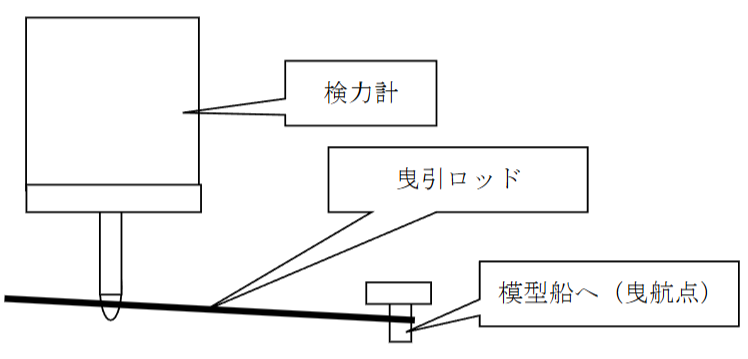
\includegraphics[width=\textwidth]{summer/ship-experiment/circulating-water-channel/load_cell_setup.png}
        \caption{検力計、曳引ロッドと曳航点の位置関係}
        \label{fig:load_cell_setup}
    \end{subfigure}
    \caption{計測装置関連図}
\end{figure}

\section{使用模型船}
本実験では、Series60 $(C_{B}=0.6)$ 船型と呼ばれるものの模型船を使用した。なお、この模型船の船首部には、乱流促進装置(Stud) が取り付けてある。
主要目を表\ref{tab:model_ship_particulars}に示す。

\begin{table}[htbp]
    \caption{模型船主要目}
    \label{tab:model_ship_particulars}
    \centering
    \begin{tabular}{|l|l|}
    \hline
    \textbf{Item} & \textbf{Series60 $(C_{B}=0.6)$} \\
    \hline
    Lpp(垂線間長) & 1 m \\
    (全幅) & 0.1333 m \\
    d(喫水) & 0.0533 m \\
    浸水表面積S & $0.1699~m^{2}$ \\
    排水量 & $4.252\times10^{-3}m^{3}$ \\
    $C_{B}$ & 0.6 \\
    A & $6.951\times10^{-3}m^{2}$ \\
    Rudder Area & $1.5\%Lpp\times D$ \\
    \hline
    \end{tabular}
\end{table}

\section{実験手順}
船舶の有効馬力を推定するために、以下の手順で実験を行った。

\begin{enumerate}
    \item 模型船にバラストウェイトを積み、規定の載貨状態に合わせた。
    \item 水温を計測した。
    \item ロードセルの検定を行った。
    \item 模型船をロードセルにセットした。
    \item 流速コントローラのインバータ周波数を適当な周波数に設定した。
    \item 定常状態になったら抵抗値、流速を測定し、船側波形の観察を行った。
    \item 5)に戻り適宜抵抗値を測定した。
    \item 水温を計測した。
\end{enumerate}

---

\chapter{結果}
抵抗試験で得られた結果を以下に示す。

\section{計測データ}
実験計画表に従って計測したデータの一部を、表\ref{tab:measurement_data_sample_booktabs}に示す。

\begin{table}[htbp]
  \centering
  \caption{計測結果}
  \label{tab:measurement_data_sample_booktabs}
  \begin{tabular}{cc}
    \toprule
    $U$ (m/s) & 計測電圧(V) \\ \midrule
    0.3       & 0.339314  \\
    0.4       & 0.558314  \\
    0.5       & 0.829342  \\
    0.6       & 1.18842   \\
    0.7       & 1.60223   \\
    0.8       & 2.10279   \\
    0.9       & 2.84873   \\
    1         & 3.67633   \\
    1.1       & 4.53782   \\ \bottomrule
  \end{tabular}
\end{table}


\section{解析結果}
解析結果については\ref{sec:kekkanobunnseki}や添付のExcelシートを参照されたい

---

\chapter{考察}
本章では、実験結果に基づき、各課題について考察する。

\section{形状影響係数Kの導出}
ロードセルの電圧データから得た全抵抗を用いて形状影響係数を求める。

全抵抗係数$C_T$を(\ref{eq:zenteikoukeisuu})式により得る
\begin{equation}
    \label{eq:zenteikoukeisuu}
    C_T=\frac{R_T}{\frac{1}{2}\rho U^2S}
\end{equation}
また、$C_{F0}$を$0.004$とし逐次代入法(\ref{eq:chikujidainyu})式により$C_F$を求める
\begin{equation}
    C_{F1} = \left( \frac{0.242}{\log_{10}(Rn \cdot C_{F0})} \right)^2 \rightarrow C_{F2} = \left( \frac{0.242}{\log_{10}(Rn \cdot C_{F1})} \right)^2 \cdots
    \label{eq:chikujidainyu}
\end{equation}

具体的な計算過程は添付の解析シートに記載する。

\section{3次元外挿法による実船の性能推定}
課題で与えられた実船の長さ $L=140 \text{m}$を想定し、上記で求めた形状影響係数$K$の値を用いて、3次元外挿法により実船の性能、すなわち有効馬力 $EHP$ を推定した。
実船の全抵抗係数 $C_{TS}$ は、
\begin{equation}
    \label{3jigengaisoho}
    C_{TS}=(1+K)C_{FS}+C_{W}+\Delta C_{F}   
\end{equation}
で求められる。\\
    ここで、$C_{FS}$ はSchönherrの式を用いて実船のレイノルズ数 $Rn_S$ から求められる摩擦抵抗係数、$C_W$ は模型試験から得られた造波抵抗係数 ($C_W = C_{WM}$)、$\Delta C_F = 0.0002$ を使用する。
そして、実船の有効馬力 $EHP$ は、
$$EHP=R_{TS}V_{S}$$
$$R_{TS}=C_{TS}\frac{1}{2}\rho_{S}S_{S}{V_{S}}^{2}$$
で計算される。具体的な計算結果は添付の解析シートに記載する。

\section{船型パラメータからのKの推定と比較考察}
prohaskaの方法で形状影響係数$k$を求めてみた。

\subsection{低速域における造波抵抗の特性}
船速が非常に遅い領域(一般的にフルード数 $F_n < 0.2$)では、造波抵抗は無視できるほど小さく、フルード数の高次のべき乗に比例すると仮定できる。

$$C_W \approx a \cdot F_n^n \quad (\text{ここで } n \ge 4) $$
上記の全抵抗係数の式を $C_F$で割ると、次のようになる。
$$\frac{C_T}{C_F} = (1+k) + \frac{C_W}{C_F} $$
ここに低速域の仮定を代入すると、
$$\frac{C_T}{C_F} \approx (1+k) + \frac{a \cdot F_n^n}{C_F} $$
この式は、縦軸に 
$\frac{C_T}{C_F}$、横軸に 
$\frac{F_n^n}{C_F}$(通常 n=4 が用いられる)をとると、直線関係になることを示している。
模型試験で得られた複数の船速(低速域)における$C_T$と、それに対応する$C_F$、および$F_n$から、各試験点について ($\frac{F_n}4{C_F}$,$\frac{C_T}{C_F}$) を計算し、グラフ上にプロットし、その線形近似曲線の切片が求めたい形状影響係数 (1+k) となる。
プロットしたグラフを以下図\ref{fig:prohaska}に記す。
\begin{figure}[H]
    \centering
    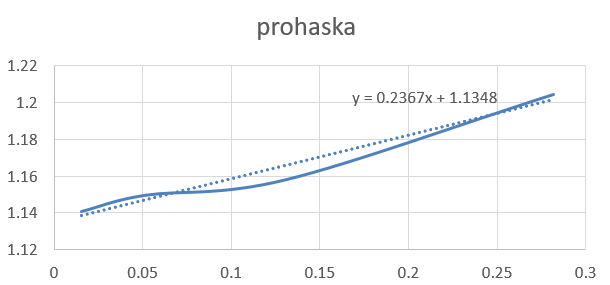
\includegraphics[width=0.5\linewidth]{summer/ship-experiment/circulating-water-channel/prohaska.png}
    \caption{Prohaskaプロット}
    \label{fig:prohaska}
\end{figure}
線形近似曲線の式は$y=0.2367x+1.1348$であり、切片の値より、$K=0.1348$となる。

参考文献:"Viscous interference analysis of trimaran vessel using computational fluid dynamic"
\url{https://www.researchgate.net/publication/371157775_Viscous_interference_analysis_of_trimaran_vessel_using_computational_fluid_dynamic}閲覧日:7/15

\section{結果の分析}
\label{sec:kekkanobunnseki}
順番が前後するが、波の観察の前にここまでで得た結果をまとめて分析していきたい。

まず、レイノルズ数と造波抵抗の関係について
\begin{figure}[H]
    \centering
    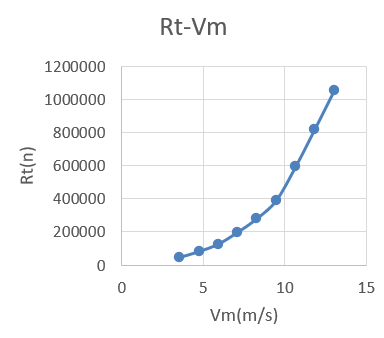
\includegraphics[width=0.5\linewidth]{summer/ship-experiment/circulating-water-channel/rt-vn.png}
    \caption{レイノルズ数と船速の関係}
    \label{fig:rt-vn}
\end{figure}
船速に対してレイノルズ数が指数関数的または累乗比例的に大きくなっていることがわかる。
このことから、船速が大きくなると船体表面の流れが層流から乱流へと変化していくと考えられる。

\vspace{5mm}

次に、レイノルズ数及びフルード数と各種抵抗係数の関係について

\begin{figure}[H]
    \centering
    \begin{subfigure}[b]{0.45\textwidth}
    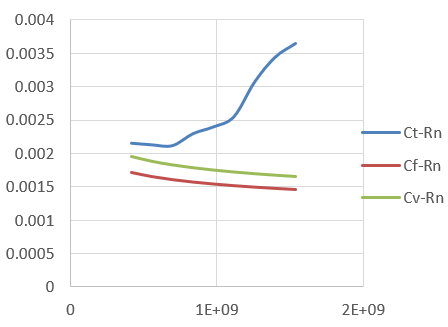
\includegraphics[width=\textwidth]{summer/ship-experiment/circulating-water-channel/c-rn.png}
        \caption{$C_T-R_n$,$C_F-R_n$,$C_V-R_n$}
        \label{fig:c-fn}
    \end{subfigure}
    \hfill
    \begin{subfigure}[b]{0.45\textwidth}
        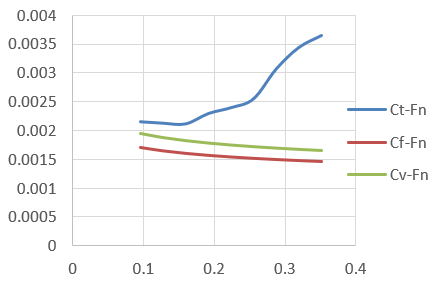
\includegraphics[width=\textwidth]{summer/ship-experiment/circulating-water-channel/c-fn.png}
        \caption{$C_T-F_n$,$C_F-F_n$,$C_V-F_n$}
        \label{fig:c-fn}
    \end{subfigure}
    \caption{レイノルズ数, フルード数と抵抗係数の関係}
\end{figure}

低速のうちは摩擦抵抗や、粘性抵抗が比較的大きい部分を占めているが、船速を上げていくにつれて造波抵抗が大きくなり、最終的に抵抗の主役となると読み取れる。特に、ある点を境に急激に造波抵抗が増加していることが読み取れる。

\vspace{5mm}

ここで、造波抵抗とフルード数の関係に注目してみたい。

\begin{figure}[H]
    \centering
    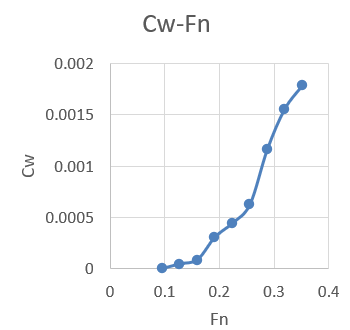
\includegraphics[width=0.5\linewidth]{summer/ship-experiment/circulating-water-channel/cw-fn.png}
    \caption{造波抵抗係数とフルード数の関係}
    \label{fig:cw-fn}
\end{figure}

フルード数が0.2までの間は造波抵抗はさほど大きくはないが、それ以上の所では造波抵抗が跳ね上がっていることがわかる。

\vspace{5mm}

最後に今回で最も重要な\textbf{馬力と船速の関係}を見てみることにする。

\begin{figure}[H]
    \centering
    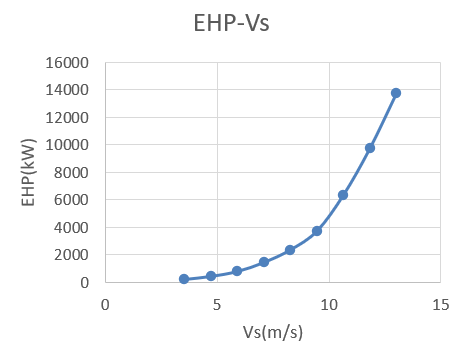
\includegraphics[width=0.5\linewidth]{summer/ship-experiment/circulating-water-channel/ehp-vs.png}
    \caption{馬力と船速の関係}
    \label{fig:ehp-vs}
\end{figure}

グラフからなめらかな曲線で船速が上がるにつれて急激に馬力が増加していることがわかる。
これは先述のとおり船速が上がるにつれて造波抵抗が急激に増加する事に起因すると考えられる。つまり、速く動かすには相応のエンジンを搭載する必要があるのである。


\section{波形と造波抵抗の関係}
回流水槽の流速を変える事で疑似的に船速を調節し、その時の波形を観察した。
\begin{figure}[H]
    \centering
    \begin{subfigure}[b]{0.45\textwidth}
    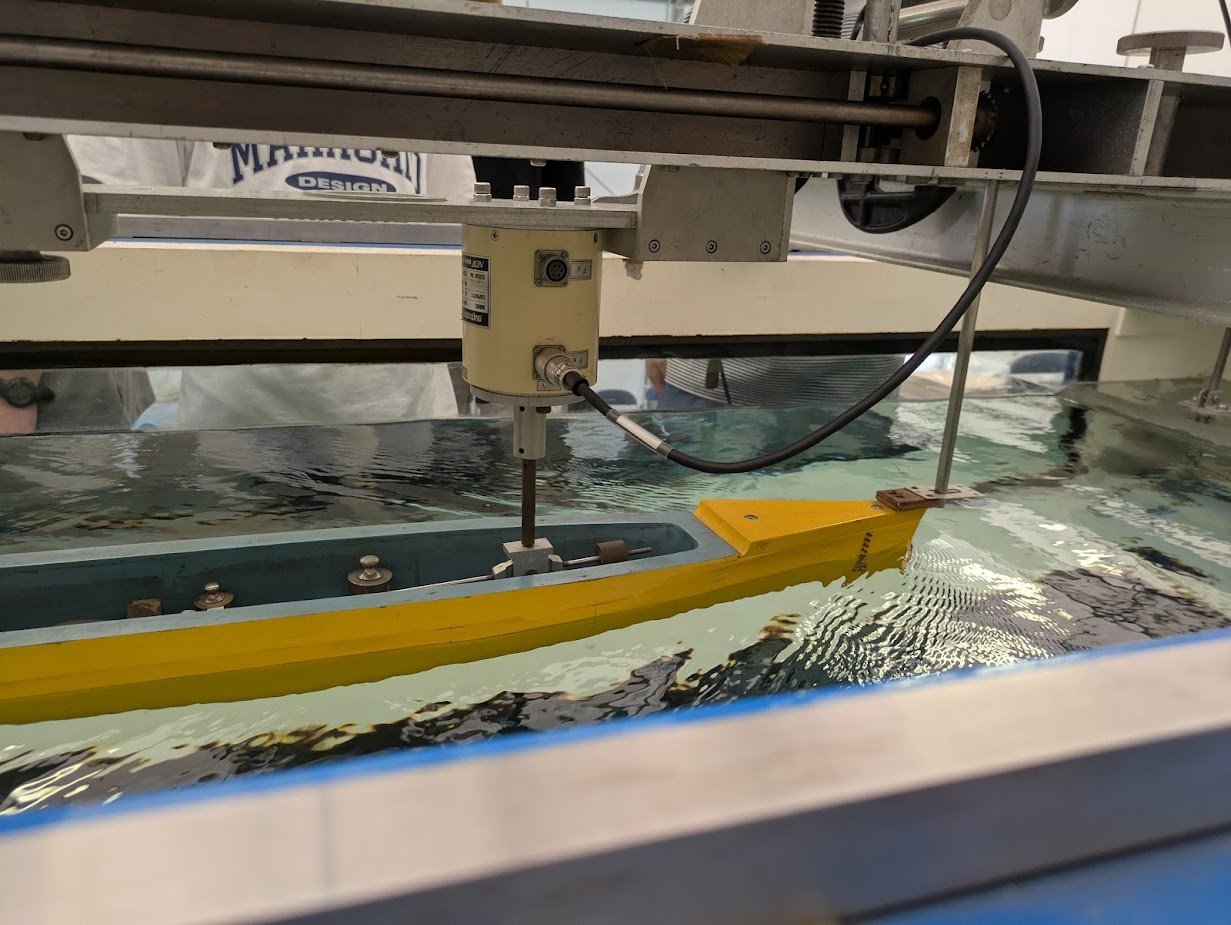
\includegraphics[width=\textwidth]{summer/ship-experiment/circulating-water-channel/teisoku.png}
        \caption{低速域での波形}
        \label{fig:teisoku}
    \end{subfigure}
    \hfill
    \begin{subfigure}[b]{0.45\textwidth}
        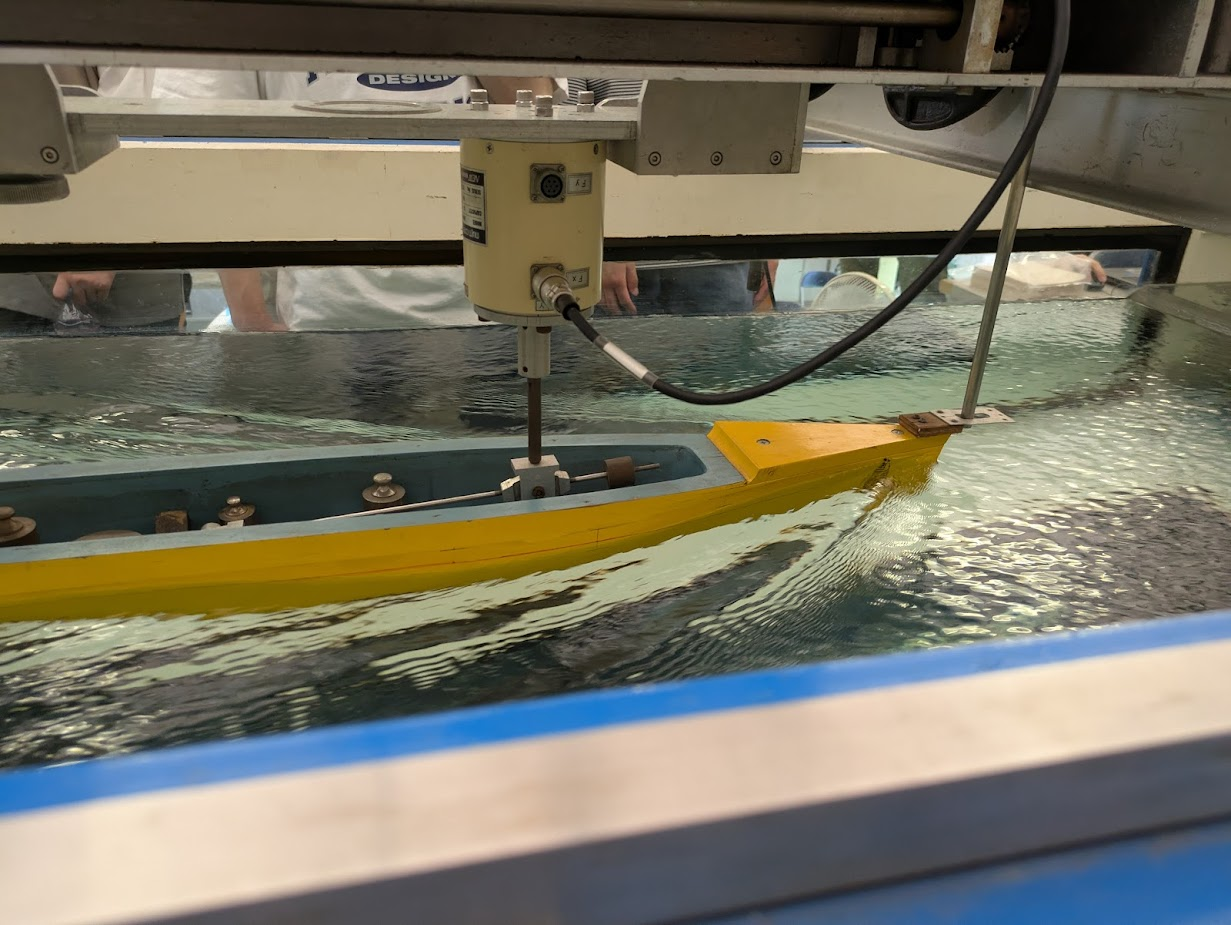
\includegraphics[width=\textwidth]{summer/ship-experiment/circulating-water-channel/kousoku.png}
        \caption{高速域での波形}
        \label{fig:kousoku}
    \end{subfigure}
    \caption{船速による波形の変化}
\end{figure}
低速時に比べて高速時には波が高くくっきり観察できる。これは\ref{sec:kekkanobunnseki}で述べた、船速が上がるほど造波抵抗が大きくなるという分析結果と合致する。

\section{全体的な考察}
今回の回流水槽を用いた抵抗試験では、模型船の抵抗を計測し、そのデータから実船の有効馬力を推定するという一連の流れを体験した。流れる水の中に模型を固定して計測するという手法は、長水槽とは異なるアプローチであり、興味深いものであった。
1+Kを用いた3次元外挿法を実際に数値として扱うことで、その理論的背景への理解が深まった。ただし、Schönherrの式や$\Delta C_F$の値など、経験的な係数を使用する部分があるため、これらの係数が実際の船舶の性能に与える影響については、さらに詳細な検討が必要である。
レポート作成において、解析結果を図としてまとめる作業は時間を要するが、グラフ化することでデータ間の関係性が視覚的に明確になり、分析の助けとなった。
今後の課題としては、形状影響係数 $K$ の推定方法をさらに掘り下げ、本実験で導出した値との比較考察を厳密に行い、差異が生じる原因を論理的に説明できることを目指したい。また、船側波形と造波抵抗の関係をより定量的に分析できるようになれば、さらに精度の高い性能推定が可能になると考えられる。

---

\chapter{参考文献}
\begin{itemize}
    \item 令和7年度 海洋工学実験資料(抵抗試験実施要領).
    \item "Viscous interference analysis of trimaran vessel using computational fluid dynamic"
\url{https://www.researchgate.net/publication/371157775_Viscous_interference_analysis_of_trimaran_vessel_using_computational_fluid_dynamic}閲覧日:7/15
\end{itemize}
\end{document}
---